\let\negmedspace\undefined
\let\negthickspace\undefined
\documentclass[journal]{IEEEtran}
\usepackage[a5paper, margin=10mm, onecolumn]{geometry}
%\usepackage{lmodern} % Ensure lmodern is loaded for pdflatex
\usepackage{tfrupee} % Include tfrupee package

\setlength{\headheight}{1cm} % Set the height of the header box
\setlength{\headsep}{0mm}     % Set the distance between the header box and the top of the text

\usepackage{gvv-book}
%\usepackage{gvv}
\usepackage{cite}
\usepackage{amsmath,amssymb,amsfonts,amsthm}
\usepackage{algorithmic}
\usepackage{graphicx}
\usepackage{textcomp}
\usepackage{xcolor}
\usepackage{txfonts}
\usepackage{listings}
\usepackage{enumitem}
\usepackage{mathtools}
\usepackage{gensymb}
\usepackage{comment}
\usepackage[breaklinks=true]{hyperref}
\usepackage{tkz-euclide} 
\usepackage{listings}
\usepackage{gvv}                                        
\def\inputGnumericTable{}                                 
\usepackage[latin1]{inputenc}                                
\usepackage{color}                                            
\usepackage{array}                                            
\usepackage{longtable}                                       
\usepackage{calc}                                             
\usepackage{multirow}                                         
\usepackage{hhline}                                           
\usepackage{ifthen}                                           
\usepackage{lscape}
\begin{document}

\bibliographystyle{IEEEtran}

\title{2.10.46}
\author{EE25BTECH11017 - Mahesh Chollangi.}
{\let\newpage\relax\maketitle}

\renewcommand{\thefigure}{\theenumi}
\renewcommand{\thetable}{\theenumi}
\setlength{\intextsep}{10pt}

\numberwithin{figure}{enumi}
\renewcommand{\thetable}{\theenumi}

\textbf{Question:} \\
Let \(\vec{V} = 2\vec{i} + \vec{j} - \vec{k}\) and \(\vec{W} = \vec{i} + 3\vec{k}\). If \(\vec{U}\) is a unit vector, then the maximum value of the scalar triple product \(\sbrak{\vec{U} \quad \vec{V} \quad \vec{W}}\) is \dots

\solution \\

Let 
\begin{align}
\vec{V} = \myvec{2 \\ 1 \\ -1}, \quad \vec{W} = \myvec{1 \\ 0 \\ 3}, \quad \vec{U} = \myvec{U_x \\ U_y \\ U_z}, \quad \norm{\vec{U}} = 1
\end{align}

The scalar triple product is:
\begin{align}
S = \det\left(
\myvec{
U_x & 2 & 1 \\
U_y & 1 & 0 \\
U_z & -1 & 3
}
\right)
\end{align}

Expanding the determinant, we get:
\begin{align}
S &= U_x \det \myvec{1 & 0 \\ -1 & 3} - U_y \det \myvec{2 & 1 \\ -1 & 3} + U_z \det \myvec{2 & 1 \\ 1 & 0} \\
&= U_x (1 \times 3 - 0 \times (-1)) - U_y (2 \times 3 - 1 \times (-1)) + U_z (2 \times 0 - 1 \times 1) \\
&= 3U_x - 7U_y - U_z
\end{align}

As \(\vec{U}\) is unit vector,
\begin{align}
U_x^2 + U_y^2 + U_z^2 = 1
\end{align}

For a vector \(\vec{A} = \myvec{3 \\ -7 \\ -1}\), the maximum value of scalar product \(\vec{U}^\top \vec{A}\) subject to \(\norm{\vec{U}} = 1\) is \(\norm{\vec{A}}\).

Calculate
\begin{align}
\norm{\vec{A}} &= \sqrt{3^2 + (-7)^2 + (-1)^2} \\
&= \sqrt{9 + 49 + 1} = \sqrt{59}
\end{align}

Hence,
\begin{align}
\max \sbrak{\vec{U} \quad \vec{V} \quad \vec{W}} = \boxed{\sqrt{59}}
\end{align}

\begin{figure}[H]
    \centering
    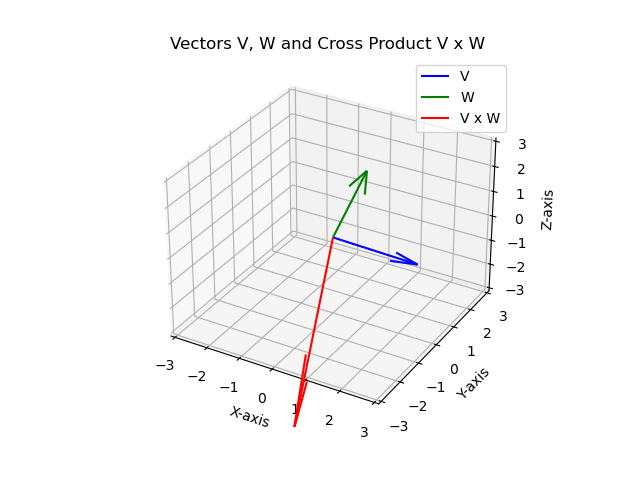
\includegraphics[width=0.8\columnwidth]{Figs/Figure_3.png}
    \caption{3D Plot}
    \label{3D Plot}
\end{figure}





\end{document}